\documentclass[a4paper,amsmath,amssymb,aps,prd]{article}
\usepackage{better_poster}
\usepackage{tikz}
\usepackage{caption}
\usepackage{subcaption}
\usepackage{graphicx}
\usepackage{geometry}

% ---- fill in from here

% authors
\title{Dynamical Analysis of Attractor Behavior in Constant Roll Inflation}
\author{William H. Kinney, Wei-Chen Lin, \textbf{Michael J. P. Morse}}

% type of poster: [exp]erimental results, [methods], [theory]
% Disclaimer: the original classification had "study" and "intervention" as separate categories. I group them under experimental results.
\newcommand\postertype{theory} % [exp],[methods],[theory]
\newcommand{\der}{\mathrm{d}}
\newcommand{\mpl}{M_{\mathrm{P}}}
\begin{document}

% main point of your study
\makefinding{
large-$\eta$ constant-roll inflation is never an attractor}

% \makemain{
% }{

% }


% the main text of your poster goes here
\makemain{
        \begin{itemize}
        \item{slow roll: $\eta \ll 1$, constant roll: $\eta = \overline{\eta} = \mathrm{Const.} \simeq 3$}
        \item{Constant roll solutions are transients, Slow Roll is attractor}
        \item{Can not inflate 60 e-folds in transient state}
        \item{Transitions to slow roll attractor in $<10$ e-folds}
        \end{itemize}
    % you can have 1 or 2 columns
    \raggedcolumns
    \setlength{\columnsep}{1cm}
   \begin{multicols}{2}
         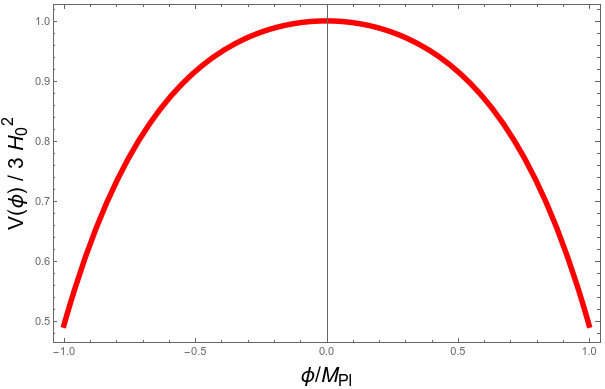
\includegraphics[width=0.7\linewidth]{images/ConcavePotential.png}
                \begin{itemize}[{}]
    \setlength\itemsep{0.1em}
        \item 
        \item
        \item
        \item
        \vspace{-2.5mm}
    \end{itemize}
        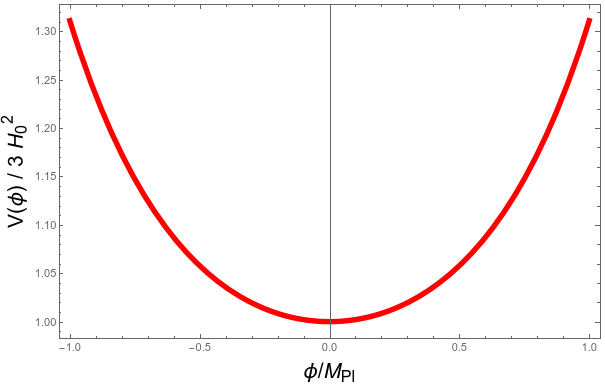
\includegraphics[width=0.7\linewidth]{images/ConvexPotential.png}      
        \columnbreak      
        
       \hspace{-2cm}
        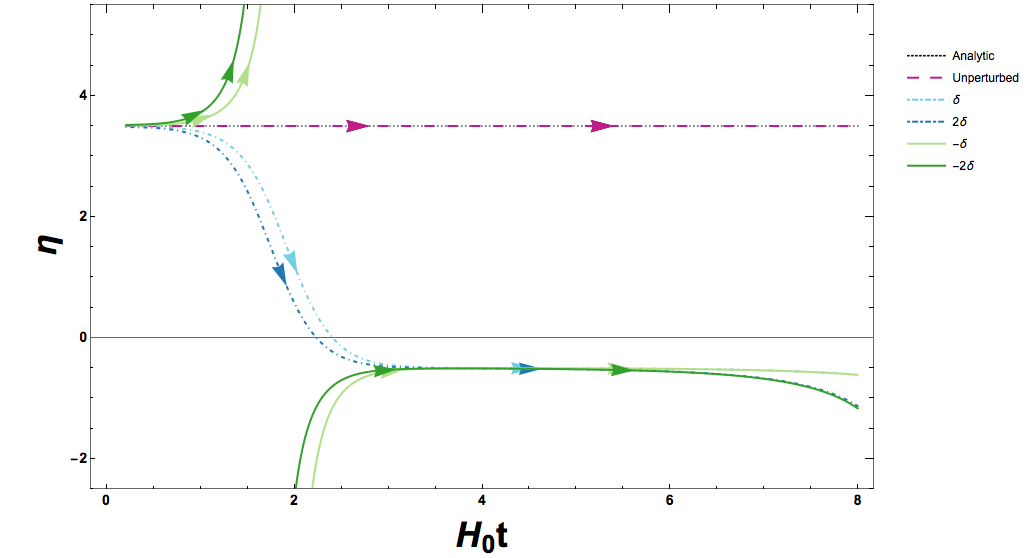
\includegraphics[width=1.4\linewidth]{images/eta_n=3_5.png}
                        \begin{itemize}[{}]
    \setlength\itemsep{0.1em}
        \item 
    \end{itemize}
         \hspace{-2cm}
        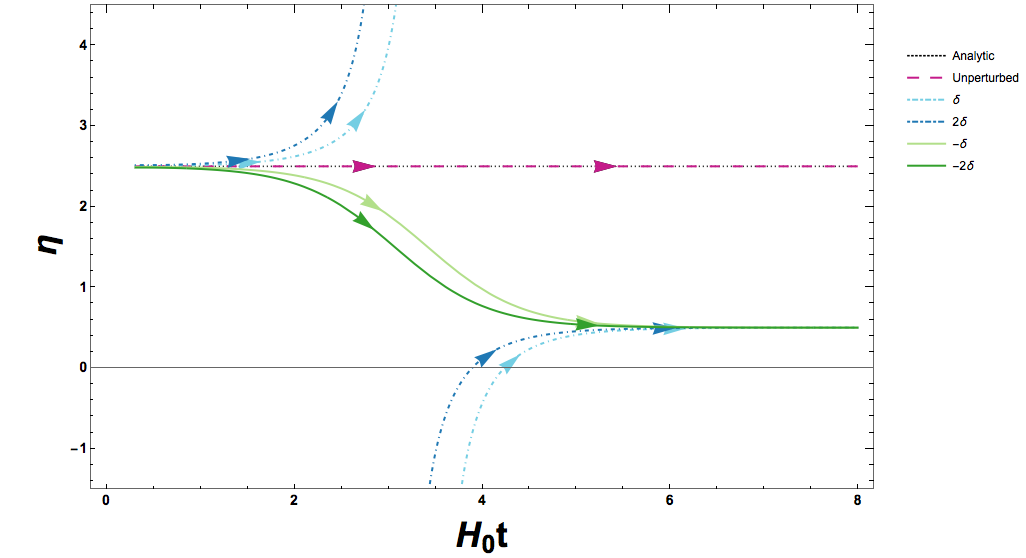
\includegraphics[width=1.4\linewidth]{images/eta_n=2_5.png}
   \end{multicols}
}
% If you have extra figures or data to show
\makeextracolumn{
    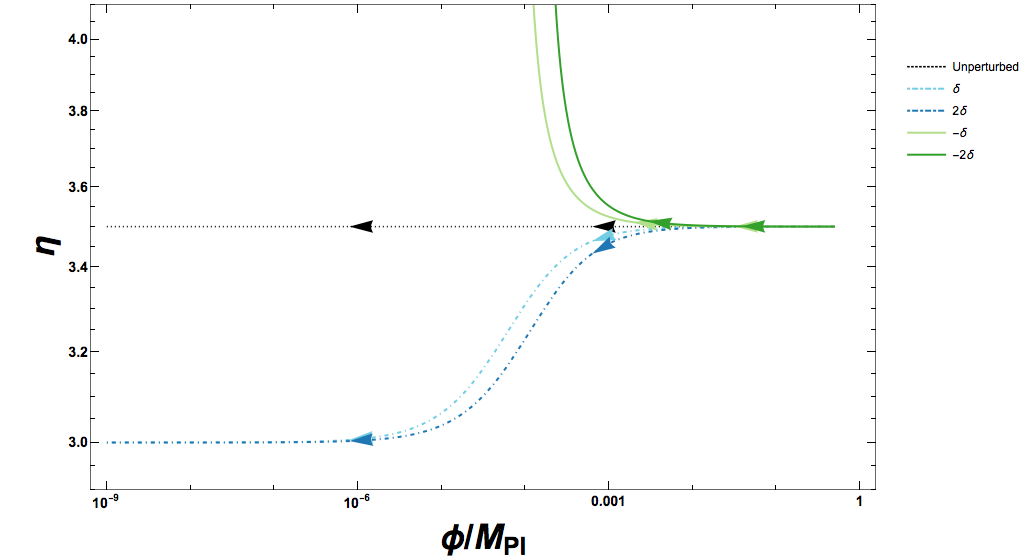
\includegraphics[width=1\linewidth]{images/eta_phi=3_5.png}
        \begin{itemize}[{}]
    \setlength\itemsep{0.1em}
        \vspace{-3mm}
        \item \hspace{2mm} Hill Top Potential $(\overline{\eta}=3.5)$
        \item
        \item
    \end{itemize}
   
    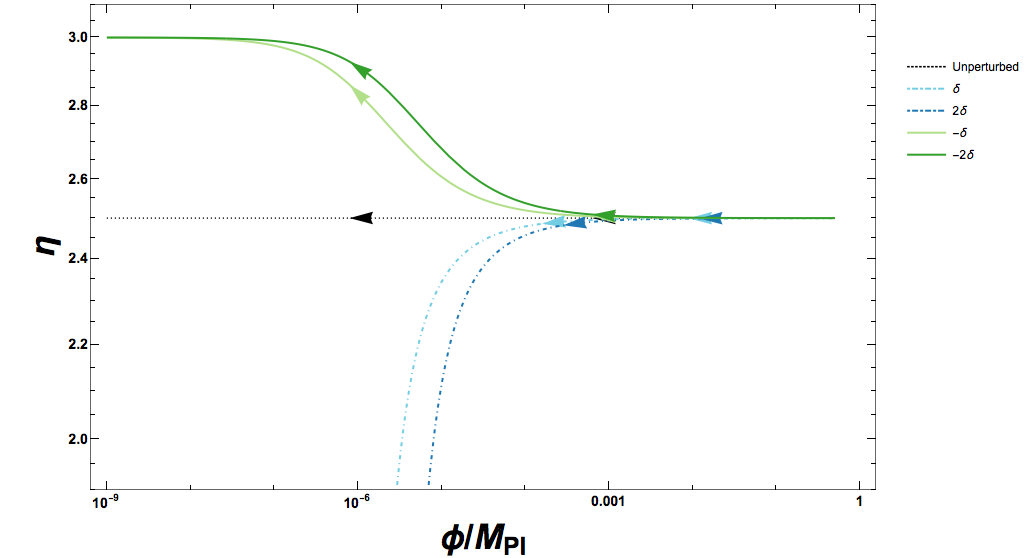
\includegraphics[width=1\linewidth]{images/eta_phi=2_5.png}
            \begin{itemize}[{}]
    \setlength\itemsep{0.1em}
         \vspace{-3mm}
        \item  \hspace{2mm} Hybrid Type Potential $(\overline{\eta}=2.5)$
        \item
        \item
    \end{itemize}
    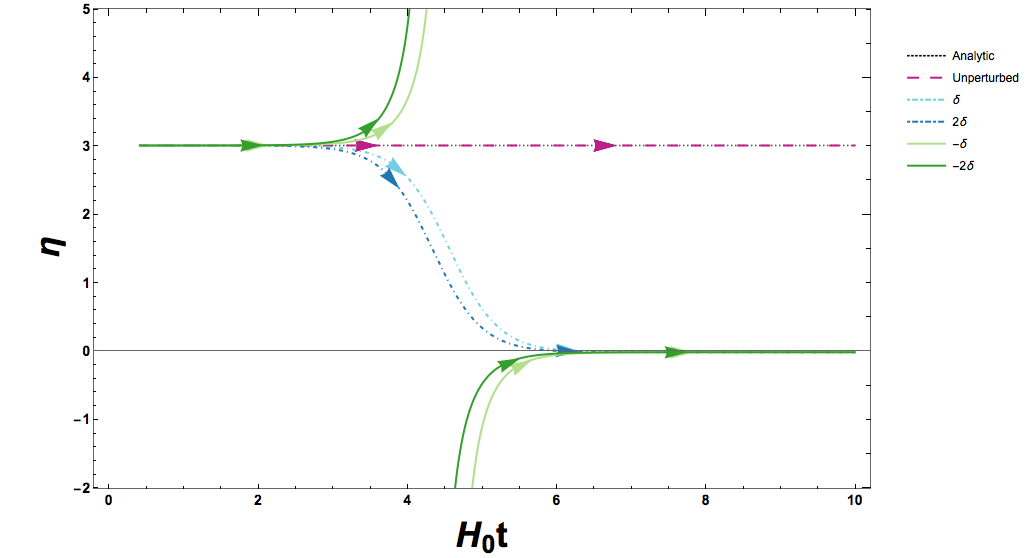
\includegraphics[width=1\linewidth]{images/eta_n=3_0115.png}  
            \begin{itemize}[{}]
    \setlength\itemsep{0.1em}
     \vspace{-3mm}
     \item{\hspace{2mm}Phenomenologically Interesting }
     \vspace{-1mm}
     \item{\hspace{2mm}Hill Top Potential $(\overline{\eta}=3.0115)$}
    \end{itemize}
}
% footer
% generate qr code from https://www.qr-code-generator.com/ and replace qr_code.png
% default: barcode on the left
\makefooter{images/Crest_BW.eps}{images/paper1.png}{images/paper2.png}


% replace with this like for barcode on the right
%\makealtfooter{images/logo.eps}{images/QR.eps}
 
\end{document}